%%%%%%%%%%%%%%%%%%%%%%%%%%%%%%%%%%%%%%%%%%%%%%%%%%%%%%%%%%%%%%%%%%
%%%%%%%% ICML 2010 EXAMPLE LATEX SUBMISSION FILE %%%%%%%%%%%%%%%%%
%%%%%%%%%%%%%%%%%%%%%%%%%%%%%%%%%%%%%%%%%%%%%%%%%%%%%%%%%%%%%%%%%%

% Use the following line _only_ if you're still using LaTeX 2.09.
%\documentstyle[icml2010,epsf,natbib]{article}
% If you rely on Latex2e packages, like most moden people use this:
\documentclass{article}
\input{/Users/joshyv/Research/misc/latex_commands.tex} 
% For figures
\usepackage{graphicx} % more modern
%\usepackage{epsfig} % less modern
\usepackage{subfigure} 

% For citations
\usepackage{natbib}

% For algorithms
\usepackage{algorithm}
\usepackage{algorithmic}

% As of 2010, we use the hyperref package to produce hyperlinks in the
% resulting PDF.  If this breaks your system, please commend out the
% following usepackage line and replace \usepackage{icml2010} with
% \usepackage[nohyperref]{icml2010} above.
\usepackage{hyperref}

% Packages hyperref and algorithmic misbehave sometimes.  We can fix
% this with the following command.
\newcommand{\theHalgorithm}{\arabic{algorithm}}

% Employ the following version of the ``usepackage'' statement for
% submitting the draft version of the paper for review.  This will set
% the note in the first column to ``Under review.  Do not distribute.''
\usepackage{icml2010} 
% Employ this version of the ``usepackage'' statement after the paper has
% been accepted, when creating the final version.  This will set the
% note in the first column to ``Appearing in''
% \usepackage[accepted]{icml2010}


% The \icmltitle you define below is probably too long as a header.
% Therefore, a short form for the running title is supplied here:
\icmltitlerunning{Submission and Formatting Instructions for ICML 2010}

\begin{document} 

\twocolumn[
\icmltitle{On utilizing structure to classify brain-graphs according to mental properties}

% It is OKAY to include author information, even for blind
% submissions: the style file will automatically remove it for you
% unless you've provided the [accepted] option to the icml2010
% package.
\icmlauthor{Your Name}{email@yourdomain.edu}
\icmladdress{Your Fantastic Institute,
            314159 Pi St., Palo Alto, CA 94306 USA}
\icmlauthor{Your CoAuthor's Name}{email@coauthordomain.edu}
\icmladdress{Their Fantastic Institute,
            27182 Exp St., Toronto, ON M6H 2T1 CANADA}

% You may provide any keywords that you 
% find helpful for describing your paper; these are used to populate 
% the "keywords" metadata in the PDF but will not be shown in the document
\icmlkeywords{boring formatting information, machine learning, ICML}

\vskip 0.3in
]

\begin{abstract} 
abstract
\end{abstract} 

\section{Introduction} % (fold)
\label{sec:introduction}


\paragraph{motivation}

Our interest is in building classifiers to operate on graphs.  In our motivating example, the graphs correspond to brains of individuals, and mental properties of those individuals are the desired classifier output.  


\paragraph{graph theory background}

erdos-renyi, p1, ERGM, stochastic blockmodels, latent feature models

\paragraph{brains as graphs background}

old skool: cajal, neural networks, PDP, 
new skool: sporns and refs

\paragraph{outline}


Section \ref{sec:def} rigorously defines the mathematical objects under investigating.  Section \ref{sec:alg} develops a number of algorithms which are proven to be asymptotically optimal under various model assumptions.  The performance of these algorithms under various simulated modeling assumptions is demonstrated in Section \ref{sec:results}.  Finally, Section \ref{sec:discussion} discusses some potential ramifications of these results, and possible directions for future work.

% section introduction (end)

\section{Definitions} % (fold)
\label{sec:def}

Our intention is to build classifiers the operate on graphs.  To proceed, we rigorous define the mathematical objects under investigation.

\subsection{Mental Properties} % (fold)
\label{sub:mental_properties}

By ``mental property'', we mean one of many possible mental properties, including intelligence level, knowledge of a certain fact or set of facts, skill level, etc.  We will investigate the relationship between brains and a \emph{single} mental property here, and leave multiple categorical classifications to future work.  Let $\mM$ be the space of all mental properties under investigation, so that $m \in \mM$.  We restrict our work here to two-way classifications, so $\mM=\{0,1\}$, corresponding to having/not having some property, or having an ability over some threshold, etc.  

% subsection mental_properties (end)

\subsection{Brain-graphs} % (fold)
\label{sub:brain_graphs}


With this in mind, we propose the notion of a \emph{brain-graph}. Specifically, we say that the brain may be well characterized as a labeled, attributed multigraph (which is a generalized notion of a or network). Formally, we define a brain-graph, $b\in \mB$ as a triple, $\mB=(\mV,\mA,\mX)$, defined by the following:
\begin{itemize}
	\item The set of vertices (nodes), $V=\{V_i\}_{i\in[N]} \in \mV \subseteq \mathbb{Z}$, where $V_i \in \{0,1\}$ for $i \in [N]=\{1,2,\ldots,N\}$, and  $\mathbb{Z}$ is the set of integers, $\{0,1,2,\ldots\}$.  
	\item The set of arcs (edges), $A=\{A_{ij}\}_{i,j \in [N]} \in \mE \subseteq \mathbb{Z}^{N^2}$. Implicitly, the above definition allows for multiedges, i.e.,  $A_{ij}: \Omega \mapsto \mathbb{Z}\, \forall \, i,j$. 
	\item The set of vertex features, $X=\{X_i\}_{i\in[N]} \in \mX \subseteq \Real^{d \times N}$, and $d$ is the countable dimensionality of the feature vectors. 
\end{itemize}

Throughout, we assume $n$ is known a priori, and the vertices are \emph{labeled}.  Further, we assume that both edges and features are random variables, but only edges are observed.  Thus, we denote a random brain-graph $b=(a,x)$, where $a=\{a_{ij}\}_{i,j \in [N]}$, and $x=\{x_i^k\}_{i\in[N], k \in [d]}$.  The class-conditional probability distributions are therefore be defined by $F_{B|M}=P[B | M]=P[A,X|M]$.  


% subsection brain_graphs (end)



% section definitions (end)


\section{Classifiers} % (fold)
\label{sec:classifiers}

If we knew $F_{B|0}$ and $F_{B|1}$, then classification would be trivial, let $\hm=\argmax_{m=0,1} \{F_{B|0}, F_{B|1}\}$.   However, in practice these distributions are typically unknown. Therefore, we must estimate $g$ from a corpus data. Assume we have collected $N$ brain/mental pairs. Then, define the corpus of data as the collection of all such pairs: $\mD_{N}=\{(b^1,m^1), \ldots, (b^n,m^n)\}$. The estimated classifier, $\hg$, then takes a new brain and the old \emph{training data}, and makes predictions about the mental property $m$. Formally, $\hg: \mB \times (\mB, \mM)^n \mapsto \mM$, so $\hg(b; \mD_n)=\hm$.  The goal is to find the classifier, $\hg \in \mG$, that minimizes some loss function, $L$, given the data.  For two-way classification, a potentially reasonable loss function is $L_F(\hg)=\mathbb{E}[P_F(\hg(B;\mD_n) \neq M | \mD_n)]$.  

Below, we describe several different graph classification algorithms that we will apply to simulated data.  Each algorithm is built explicitly with some model assumptions in mind.  As the number of constraints increase, the bias of the classifier potentially increases.  However, the variance certainly decreases.  So, if we can find an algorithm that reduces the variance more than it increases the bias, then we win the bias-variance trade-off, and have obtained the best $\hg$ we can find.  Further, comparing the various algorithmic performances' on real data will inform us with regard to which model assumptions are best supported by the data, potentially leading to greater insight and understanding of the underlying neurobiology.  

\subsection{$k_n$ nearest neighbor (kNN)} % (fold)
\label{sub:_k_n_nearest_neighbor_knn_}

The $k_n$ nearest neighbor (kNN) algorithm is was proven to be universally consistent when the data are vectors in $\Real^d$ \cite{Stone77}.  More recently, Vogelstein et al. (2009) extended this proof to the space of attributed multigraphs \cite{VVP09}.  Universality implies that no matter what $F_{B|M}$ looks like, the kNN algorithm will asymptotically converge to the Bayes optimal estimator, that is, as $N\conv\infty\, \hg \conv g_{\ast}$, where $g_{\ast}= \argmax_g L_F(g)$.  

The kNN algorithm on graphs operates as follows.  Let $d(b_i,b_j)=\norm{a_i,a_j}_F^2$, where $a_i$ is the adjacency matrix for brain $i$.  Given a new brain, $b$, compute $d(b,b_i)\, \forall i \in [n]$.  Then, sort the brains and their corresponding mental properties according to their distances from $b$: $b_{(1)}, b_{(2)}, \ldots$.  Define $S_0=\sum_{i \in [N]} I\{d(b,b_{(i)} < d(b,b_{(k_)})) | m_{(i)}=0\}$, and similarly for $S_1$. Then, $\hm=\argmax_{0,1} \{S_0,S_1\}$.  Note that no model assumptions were made, so this algorithm will work regardless of $F_{B|M}$, assuming some rule to ensure that as $n\conv \infty$, $k \conv \infty$ and $k/n \conv 0$.  We chose $k=\sqrt{c n}$, where $c$ was determined empirically to be 16.  

% subsection _k_n_nearest_neighbor_knn_ (end)


\subsection{Edge independent assumption} % (fold)
\label{sub:edge_indep}

In the above, $F_{B|M}$ was not explicitly specified, as the kNN algorithm is model-free and non-parametric.  Here, we assume that each edge is independent, conditioned on the class:
\begin{align}
	P[B|M]=P[A|M]=\prod_{i,j \in [N]} P[A_{ij} | M]
\end{align}
To utilize such a model, a precise distribution for $P[A_{ij}|M]$ must be specified.  A natural choice is a Poisson distribution, thus:
\begin{align}
	P[A_{ij}=a_{ij} |M=m]=\text{Poisson}(a_{ij}; \lam_{ij,m}) = \frac{\lam_{ij,m}^{a_{ij} \text{e}^{\lam_{ij,m}}}}{a_{ij}!}
\end{align}
Note that this is a generalization of an Erdos-Renyi graph, where each binary edge is independent but sampled from the same Bernoulli distribution with probability $p$.  The above implies that the class conditional distributions are governed entirely by $\Lam_m=\{\lam_{ij,m}\}_{ij \in [N]}$.  

To use this classifier in practice, we first compute the maximum likelihood estimate of the parameters $m=0$:
\begin{align}
	\hlam_{ij,0} = \frac{1}{n_0}\sum_{l | m^l = 0} a_{ij}^l
\end{align}
where $n_0$ is the number of training samples in class $0$, and $a_{ij}^l$ is the number of edges between vertices $i$ and $j$ for brain $l$.  The same procedure may be used for $m=1$ as well, to obtain $\hLam_0$ and $\hLam_1$.  Then, given a new brain with adjacency matrix, $a$, choose $\hm$:
\begin{align}
	\hm = \argmax_{0,1} \left\{\prod_{ij \in [N]} \text{Poisson}(a_{ij}; \hLam_0), \prod_{ij \in [N]} \text{Poisson}(a_{ij}; \hLam_1)\right\}
\end{align}
In practice, it is sometimes the case that $a_{ij}^l=0 \, \forall ij \in [N]$ and $\forall m^l = 0$ or $1$, but then for the new data, $a_{ij>0}$.  In such a scenario, $\hlam_{ij,m}=0$, so $P[a_ij > 0 | \hlam_{ij,m}]=0$.  This results in a zero probability for such a graph, which is an undesirable artifact of a small sample size.  To mediate this effect, we could impose a prior on $\Lam$, such that even in the small sample size case, $0$ probabilities are less frequent.  A reasonable choice would be a Gamma distribution, which is the conjugate prior of the Poisson distribution.  However, the Gamma distribution also has 2 hyperparameters, and we do not have a reasonable way of choosing them in real data.  Thus, instead, we manually impose the following rule: if $\hlam_{ij,m}=0$, then let $\hlam_{ij,m}=1/(2 n_m)$, i.e., $\hlam_{ij,m}$ is half of what it would be if exactly one class $m$ training observation exhibited an edge between $i$ and $j$. Because of this hack, this algorithm is an approximate Naives Bayes Plug-in classifier.
% 
% \begin{align}
% 	\hlam_c &= \argmax_{\lam_c \geq 0}  \prod_{l | m^l = c} P(\lam_c | b^l) = \argmax_{\lam_c \geq 0}  \bigg(\prod_{l | m^l=c} P(b^l | \lam_c)\bigg) P(\lam_c) = \argmax_{\lam_c \geq 0}     \prod_{\substack{l | m^l = c \\ (i,j) \in E^l}} P_E(e^l_{ij} | \lam_c) P(\lam_c)\nonumber \\
% 	&= \argmax_{\lam_c \geq 0} \prod_{\substack{l | m^l = c \\ (i,j) \in E^l}}  \text{Poisson}(e^l_{ij}; \lambda_c) \text{Gamma}(\lam_c; \alpha, \beta) \nonumber \\ 
% 	&= \argmax_{\lam_c \geq 0} \prod_{\substack{l | m^l = c \\ (i,j) \in e^l}} \text{Gamma}(\lam_c; \alpha + \sum_{\substack{l | m^l = c \\ (i,j)\in e^l}} e^l_{ij}, \beta + \sum_{l \in [n]}|e^l| ).
% 	%\frac{ \lam^{E^l_{ij}}\exp\{-\lam\} }{E^l_{ij}!} \lam^{\alpha-1} \frac{\exp\{-\lam \beta \}}{\Gam(\alpha)/\beta} = \argmax_{\lam \geq 0} \prod_{\substack{l \in [n] \\ (i,j) \in E^l}} 
% \end{align}
% Once we obtain $\hth=\{\hlam_0,\hlam_1,\ldots, \hlam_C\}$, given a new brain, $b$, classifying $b$ is trivial:
% \begin{align}
% 	\hm &= g_n(b; \mD_n, \hth) = \argmax_{c \in [C]} \{P_E(b | \hlam_c)\} %\nonumber \\& 
% 	= \argmax_{c\in[C]} \prod_{(i,j)\in e}\text{Poisson}(e_{ij}; \hlam_c).
% \end{align}
% This strategy, of course, can be easily generalized in a number of ways.  First, $\lam$ could be a function of edge identity, instead of the same across all edges.  Second, the hyperparameters could be different across classes.  Third,  the hyperparameters can be estimated using, for instance, cross-validation.  Note that for numerical reasons, we typically use log posteriors, requiring a summation instead of multiplication of many potentially small numbers.
% 
% 
% Unfortunately, while tractable and simple, this model does not satisfy all of our above desiderata with respect to $\mP$.  In particular, this is a \emph{parametric} model, meaning that the number of parameters is necessarily \emph{finite} ($\leq n^2$).  Thus, while this model can act as a \naive base model, more sophisticated models are desirable.


% subsubsection edge_independent_models (end)

\subsection{Edge independent and reduced subspace contains signal} % (fold)
\label{sub:edge_independent_and_reduced_subspace_contains_signal}

The above algorithm operates on the full parameter space, $\Lam$.  Each class conditional parameter lives in a $N^2$ dimensional space: $\Lam_m \in \Real_+^{N^2}$.  It is often the case, however, that much of the signal lives in a much lower dimensional space.  However, a priori, the particular canonical low-dimensions are unknown.  Therefore, some dimensionality reduction technique is required.  We compute the difference matrix: $\hLam_{\Delta}=|\hLam_0 - \hLam_1|$.  Large elements of $\hLam_{\Delta}$ indicate that the two class conditional distributions differ drastically, and small elements of $\hLam_{\Delta}$ indicate that the class conditional distributions are nearly the same.  To reduce the dimensionality of the problem, we first collapse $\hLam_{\Delta}$ into a vector, and then sort it from highest to lowest, and call the result $\hS_{\Delta}$.   We then plot $\hS_{\Delta}$ to ``find the elbow'', that is, find the inflection point in the plot that potentially divides those elements with signal from those elements that are noise.  


% subsection edge_independent_and_reduced_subspace_contains_signal (end)


\subsection{Edge independent and coherence} % (fold)
\label{sub:edge_independent_and_coherence}

% subsection edge_independent_and_coherence (end)


\subsection{Edge independent and semi-coherent} % (fold)
\label{sub:edge_independent_and_semi_coherent}

% subsection edge_independent_and_semi_coherent (end)

\subsection{Edge conditionally independent} % (fold)
\label{sub:edge_cond}


In Section \ref{ssub:edge_indep}, we defined a very simple model, completely neglecting all features, and assuming the each edge is independent.  For many data sets, making either of these assumptions (and all the more so for both of these assumptions) will not yield satisfactory descriptions of the data \cite{?}.  Here, we relax the last two assumptions.  Rather, the probability of each edge is only a function of the feature vectors for the two vertices that define the edge, and the feature vector of the edge.  In this model, edges are not independent, but they are \emph{conditionally independent} given the features.   Formally, denote vertex features by $x_v=(x_1, \ldots, x_{n})$ and denote edge features by $x_e=(x_{1,1}, \ldots, x_{1,n}, x_{2,1}, \ldots x_{n,n})$, so the total feature vector for a brain-graph is $x=(x_v, x_e)$.  Then, the brain-graph is characterized entirely by $b=(e,x)$, and for any brain-graph, one can write:
\begin{align}
	P(b^l | \theta) &= P(e^l, x^l | \theta) = P_E(e^l | x^l) P_X(x^l | \theta) 
\end{align}
Assuming that all edges and features are observed, and we have classes $\{0,1,\ldots,C\}$, yielding conditional parameters, $\{\theta_0$, $\theta_1$, $\ldots$, $\theta_C\}$, then we can estimate the parameters for this model, for any particular class $c$:
\begin{align}
\widehat{\theta}_c 	&= \argmax_{\theta_c \in \Theta} \prod_{l | m^l=c} P(\theta_c | e^l, x^l) %\nonumber \\ &
		= \argmax_{\theta_c \in \Theta} \prod_{l | m^l=c} P(e^l, x^l | \theta_c) P_{\theta}(\theta_c) \nonumber \\
		&= \argmax_{\theta_c \in \Theta} \prod_{l | m^l=c} P_E(e^l | x^l) P_X(x^l | \theta_c) P_{\theta}(\theta_c) 					 					
		= \argmax_{\theta_c \in \Theta} \prod_{l | m^l=c}  P_X(x^l | \theta_c) P_{\theta}(\theta_c).  \label{eq:cond}
\end{align}
To solve Eq.~\ref{eq:cond}, we must only specify both $P_X$ and $P_{\theta}$, but not $P_E$.  However, the nature of $P_E$ will impact the other decisions, so we therefore specify it as well.  Because the data under consideration are integer weighted edges, a natural choice for $P_E$ is a Poisson distribution, with some rate, $\lam \geq 0$:
\begin{align} \label{eq:E}
	P_E(e_{ij} | x_i,x_j) = \text{Poisson}(e_{ij}; f(\langle x_i, x_j \rangle))
\end{align}
where $\langle \cdot, \cdot \rangle$ indicates a dot product, and $f$ is some ``link'' function.  Note that the dependence on edge features, $x_{ij}$, has been dropped.  The link function here plays the role of mapping the dot product into the support of Poisson rates, which is non-negative (similar to the link function in a generalized linear model \cite{McCullaghNelder89}).  We consider two possibilities for $x$.

\paragraph{$x \in \Real^d_+$}

If $x$ lives in some space such that $\langle x_i, x_j \rangle \geq 0$ for all $x_i, x_j \in \mX_V$, then $f$ can be a simple identity function.  One example of such a space is the unit hypercube \cite{?}. The parameters governing this distribution, $\vmu$, $\sig$, and $\alpha$ control the frequency, variability and correlation of $x$, respectively. 

sampling $x$

estimating parameters

conjugate prior

(waiting to get the pre-print on hypercube distributions).  

\paragraph{$x \in \Real^d$}

However, if $x$'s live in some more general space, such as $\Real$, then $f$ can be an exponential function.  In such a scenario, $x$ can be sampled from a multivariate Gaussian distribution, that is $P_X( \cdot | \theta)=\mN(\cdot; \mu,\Sigma)$.  Ignoring the prior $P_{\theta}$, we can use standard tools to compute the maximum likelihood estimate (MLE) of $\theta_c$:
\begin{align}
	\hmu_c &= \argmax_{\mu_c} \prod_{l | m^l= c} \mN(x^l; \mu_c, \Sigma_c) = \frac{1}{n_c} \sum_{l | m^l = c} x_l \\
	\hSig_c &= \argmax_{\Sig_c} \prod_{l | m^l= c} \mN(x^l; \mu_c, \Sigma_c) =\frac{1}{n_c} \sum_{l | m^l=c} (x^l - \hmu_c) (x^l -\hmu_c)\T.
\end{align}
Alternately, the Normal-Inverse-Wishart distribution is the conjugate prior of the Gaussian distribution, so we could incorporate prior information. In practice, incorporating prior information will typically be required, as $\theta_c \in \Real^d$ is far too high-dimensional to estimate from typical data sets, since $d \geq n^2+n$.  Thus, we can incorporate strong prior knowledge in a number of ways.  First, we assume that vertex and edge features are independent, meaning $\Sig_c$ is block-diagonal.  We can make $\Sig_c$ more ``blocky'' by assuming vertex features are independent of one another, and similarly for edge features.  This yields an independent covariance matrix for each feature vector.  Then, we can assume that each feature vector has a diagonal covariance matrix. More strongly, we can assume each covariance matrix is a scalar times the identity matrix.  If we are feeling really saucy, we could even assume that the covariance matrices are known.  

\paragraph{Choosing $\hd$}

For both the above choices, this model can satisfy all the above criteria for $\mP$, assuming that $d$ is allowed to increase to infinity.  Both semiparameter and nonparameter approaches could be used to choose $\hd$.  Cross-validation, AIC, BIC, or many other methods may be used to determine the optimal $\hd$ from the data. 


\paragraph{Classifying}

Letting $\theta=\{\theta_0,\ldots,\theta_C\}$, once $\hth_c \in \Real^{\hd}$ is estimated for each $c\in[C]$, we classify a new brain $b=(e,x)$ according to:
\begin{align}
	 \hm &= g_n(b; \mD_n, \theta) = \argmax_{c\in[C]} P(b | \theta_c) 
	 	 = \argmax_{c\in[C]}  P_E(e | x)  P_X(x | \theta_c) P_{\theta}(\theta_c) \nonumber \\
		&= \argmax_{c\in[C]}  \bigg(\prod_{i,j \in [n]} P_E(e_{ij} | x_i, x_j, x_{ij}) P_X(x_{ij} | \hth_{c_{ij}})\bigg) \bigg(\prod_{i \in [n]} P_X(x_i | \hth_{c_i})\bigg)  P_{\theta}(\hth_c)
		,
\end{align}
where we have assumed that $P_E(x_i | \theta_c)=P_E(x_i | \theta_{c_i})$ for all $i$.


\paragraph{Unobserved features, but known parameters}

In the above, we implicitly assumed that all the edges and features were observed.  In practice, however, this is often not the case.  Assume, for the moment, that $e$ \emph{and} $\theta$ are known, but $x$ is not known.  Then, we have:
\begin{align} \label{eq:hx}
	\hx &= \argmax_{x \in \mX} P(x|e;\theta) = \argmax_{x \in \mX} P(e|x;\theta) P_X(x|\theta) = \argmax_{x \in \mX} 
	 P_E(e|x) P_X(x|\theta) \nonumber \\
	&= \argmax_{x \in \mX} \prod_{i,j \in [n]} P_E(e_{ij}|x_i,x_j) P_X(x_i | \theta_i) P_X(x_j|\theta_j) \nonumber \\
	&= \argmax_{x \in \mX} \sum_{i,j \in [n]} \ln P_E(e_{ij}|x_i,x_j) + \ln P_X(x_i | \theta_i) + \ln  P_X(x_j|\theta_j) 
	% &= \argmax_{x \in \mX} \ln P_E(e|x) + \ln P_X(x | \theta)
\end{align}
where the first equality follows from applying Bayes rule twice and dropping terms that do not depend on $x$, and the second equality comes from our model assumptions.  Substituting Eq.~\eqref{eq:E} and letting $P_X$ be a Gaussian, Eq.~\eqref{eq:hx} simplifies:
\begin{align} \label{eq:hx2}
	\hx &= \argmax_{x \in \mX} \sum_{i,j \in [n]} e_{ij} - \exp\{x_i\T x_j\} - \ln (e_{ij}!) - \sum_{k=i,j} \ln \big((2\pi)^{d/2} |\Sigma_k|^{1/2}\big) - \frac{1}{2} (x_k-\mu_k)\T \Sigma_k^{-1} (x_k-\mu_k) \nonumber \\
	&= \argmax_{x \in \mX} \sum_{i,j \in [n]} -\exp\{x_i\T x_j\} - \sum_{k=i,j}\frac{1}{2} (x_k-\mu_k)\T \Sigma_k^{-1} (x_k-\mu_k)
\end{align}
where the second equality comes from dropping terms independent of $x$.  Seems to me like everything is now concave in $x$, so we can use gradient ascent to obtain $\hx$.  I haven't checked yet though, and it seems a little too good to be true.




\paragraph{Unobserved features, and unknown parameters}

In practice, often neither the features $x$, nor the parameters, $\theta$, are known a priori.  Thus, our goal is to jointly infer $x$ and $\theta$.  Three strategies are ``natural'': (i) an expectation-maximization (EM) strategy, in which one alternates computing the expected value of $x^h$, and using that expected value to maximize the estimate of $\theta$, (ii) a Gibbs sampling approach, in which we recursively sample from each to build up the joint distribution, (iii) an approximate EM approach where instead of computing the full expectation, we only compute the MAP estimate.  Assuming we can obtain $\hx$, we can plug it in to update $\hth$, and recurse.

\subparagraph{EM strategy}

To use the EM strategy, assume for the moment that edges are all observed, but features are not.  Therefore, the EM approach proceeds in two steps:
\begin{align*}
\textbf{E step: } \text{Compute } & Q(\theta,\theta') = E_{P(x | e; \theta')} \ln P(e,x | \theta) = \int P(x | e; \theta') \ln P(e,x | \theta) dx\\
\textbf{M step: } \text{Compute }& \hth = \argmax_{\theta} Q(\theta,\theta')
\end{align*}
Note that $P(e,x|\theta)$ factorizes:
\begin{align}
	P(e,x|\theta) &= P(e | x; \theta) P(x | \theta) = P(e|x) P(x|\theta) = \prod_{ij} P(e_{ij} | x_i,x_j) P(x_i, x_j | \theta) \nonumber \\ 
	&=  \prod_{ij} P(e_{ij} | x_i,x_j) P(x_i| \theta_i) P(x_j | \theta_j)
\end{align}
Further, $P(x|e;\theta)$ also factorizes:
\begin{align}
	P(x|e;\theta) &= \prod_{ij} P(x_i, x_j | \vec{e}_{ij}, \theta_{ij} )
\end{align}
where $\vec{e}_{ij}=\{\ve{e}_{i\cdot}, e_{\cdot i}, e_{j\cdot}, e_{\cdot j}\}$, where we introduce notation $e_{i\cdot}=[e_{i,1}, \ldots, e_{i,n}]$, and $\theta_{ij}=[\theta_i,\theta_j]$.  Therefore, we can expand $Q$:
\begin{align}
	Q(\theta,\theta') = \iint \prod_{i,j \in [n]} P(x_i,x_j | \vec{e}_{ij}; \theta_{ij}) [\ln P(e_{ij}| x_i, x_j) + \ln P(x_i | \theta_i) + \ln P(x_j | \theta_j)] dx_i dx_j
\end{align}
If $P(x|\theta)$ is Gaussian, then we can approximate $P(x_i,x_j | \vec{e}_{ij}; \theta_{ij})$ as a Gaussian, and maybe the same for $P(e_{ij} | x_i,x_j)$, and then maybe something good happens?



\paragraph{Kidney and egg like special case}

only a small set of vertices change their features.  fit the model assuming two classes.  compute  $D(P_X(x_i | \theta_0) || P_X(x_i | \theta_1))$ for all $i$.  rank them, and call them $x_{(1)}, \ldots, x_{(n)}$.  fit the model assuming that every vertex except $x_{(1)}$ comes from a one class model, but fit $x_{(1)}$ to a two-class model.  cross-validate to see how well that works.  re-rank vertices using the same metric, based on this new model.  repeat, adding another vertex to the two-class case, until we stop getting improvements.

%$x_i \sim P_X(\cdot | \theta_i)$ for all $x_{(i)}$ where $i \in \{2,\ldots, n\}$, but $x_{(1)} \sim P_X(\cdot | \theta_)$

% section classifiers (end)


\section{Results}  % (fold)
\label{sec:results}

To evaluate the various above described algorithms, we use each approach on simulated data.  In particular, XXX here we place the simulation from our supervenience paper XXX:

% As an example of a feasible experiment, one may consider a species whose nervous system consists of the same (small) number of labeled neurons for each organism. {\it Caenorhabditis elegans} is believed to be such a species \cite{Durbin87}. The hermaphroditic C.~elegans' somatic nervous system consists of 279 interconnected neurons. While the graph with these neurons as vertices and edges defined by chemical synapses between neurons is not identical across individuals, it is reasonably consistent \cite{Durbin87}. Furthermore, these animals exhibit a rich behavioral repertoire that depends on circuit properties \cite{deBonoMaricq05}. Thus, one may design an experiment by describing the joint distribution $F_{BM}$ via class-conditional distributions $F_{B|M=m_j}$ for the C.~elegans brain-graph for two mental properties of interest, $m_0$ and $m_1$, along with the prior probability of class membership $P[M=m_1]$. Here the mental property corresponds to the C.~elegans exhibiting or not exhibiting a particular behavior (e.g., response to an odor).
% 
% Simulations suggest that one may build a classifier, practically and with a manageable training sample size $n$, that demonstrates $\varepsilon$-supervenience with reasonable choices for $\varepsilon$ and $\alpha$ and a plausible joint distribution $F_{BM}$ (Figure \ref{fig1}). To generate the data, we let the class-conditional random variable $E_{ij} | M=m_0$ be distributed Poisson$(A_{ij}+\eta)$, where $A_{ij}$ is the number of chemical synapses between neuron $i$ and neuron $j$ according to \cite{VarshneyChklovskii09}, with noise parameter $0<\eta \ll 1$. The class-conditional random variable $E_{ij} | M=m_1$ is distributed Poisson$(A_{ij}+ k_{ij})$ for neurons $i,j \in \mD$, where $\mD$ is the set of edges deemed responsible for odor-evoked behavior according to \cite{ChalasaniBargmann07}, with signal parameter $k_{ij}$ uniformly sampled from $[-5,5]$. We consider $k_n$-nearest neighbor classification of labeled multigraphs (directed, with loops) on 279 vertices, under Frobenius norm. The $k_n$-nearest neighbor classifier used here satisfies $k_n \rightarrow \infty$ as $n \rightarrow \infty$ and $k_n/n \rightarrow 0$ as $n \rightarrow \infty$, ensuring universal consistency. (Better classifiers can be constructed for the joint distribution $F_{BM}$ used here; however, we demand universal consistency.)
% 
% Importantly, conducting this experiment {\it in actu} is not beyond current technological limitations. 3D superresolution imaging \cite{VaziriShank08} combined with neurite tracing algorithms \cite{HelmstaedterDenk08,Mishchenko09,LuLichtman09} allow the collection of a brain-graph within a day. Genetic manipulations, laser ablations, and training paradigms can each be used to obtain a non-wild type population for use as $M=m_1$ \cite{deBonoMaricq05}, and the class of each organism ($m_0$ vs.~$m_1$) can also be determined automatically \cite{BuckinghamSattelle08}.

\begin{figure}[h!]
\centering 
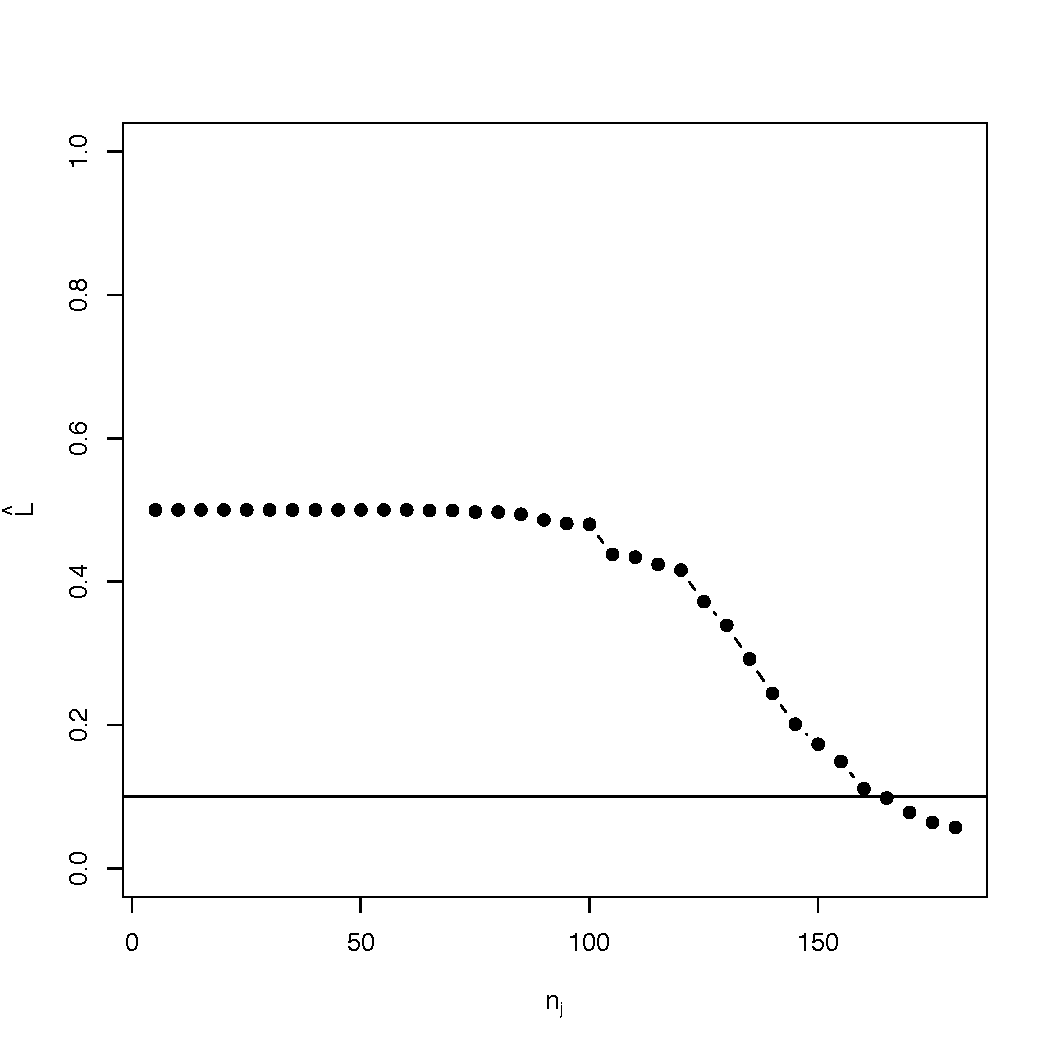
\includegraphics[width=.5\linewidth]{Lhatplot}
\caption{fig gets additional lines for additional algorithms now.  %C.~elegans graph classification simulation results. $\hL^{1000}_{F}(g_n)$ is plotted as a function of class-conditional training sample size $n_j$, suggesting that for $\varepsilon=0.1$ we can determine that $\MeB$ holds with $99\%$ confidence with just a few hundred training samples generated from $F_{BM}$. Each dot depicts an estimate for $L_{F}(g_n)$; standard errors are $(L_{F}(g_n)(1-L_{F}(g_n))/1000)^{1/2}$. E.g., $n_j = 180$ ; $k_n = 53$ ; $\hL^{1000}_{F}(g_n) = 0.057$; standard error less than 0.01. We reject $H_0: L_{F}(g^*) \geq 0.10$ at $\alpha=0.01$. $L_{F}(g^*) \approx 0$ for this simulation.
˝}
\label{fig1}
\end{figure}


% section results (end)

\section{Discussion} % (fold)
\label{sec:discussion}

% section discussion (end)

% Acknowledgements should only appear in the accepted version. 
\section*{Acknowledgments} 
 
% \textbf{Do not} include acknowledgements in the initial version of
% the paper submitted for blind review.
% 
% If a paper is accepted, the final camera-ready version can (and
% probably should) include acknowledgements. In this case, please
% place such acknowledgements in an unnumbered section at the
% end of the paper. Typically, this will include thanks to reviewers
% who gave useful comments, to colleagues who contributed to the ideas, 
% and to funding agencies and corporate sponsors that provided financial 
% support.  


% In the unusual situation where you want a paper to appear in the
% references without citing it in the main text, use \nocite
\nocite{langley00}

\bibliography{/Users/joshyv/Research/misc/biblist}
\bibliographystyle{icml2010}

\end{document} 


% This document was modified from the file originally made available by
% Pat Langley and Andrea Danyluk for ICML-2K. This 2010 version was
% created by Thorsten Joachims & Johannes Fuernkranz, 
% slightly modified from the 2009 version by Kiri Wagstaff and 
% Sam Roweis's 2008 version, which is slightly modified from 
% Prasad Tadepalli's 2007 version which is a lightly 
% changed version of the previous year's version by Andrew Moore, 
% which was in turn edited from those of Kristian Kersting and 
% Codrina Lauth. Alex Smola contributed to the algorithmic style files.  


